\documentclass[11pt]{article}
\usepackage{fullpage}
\usepackage{listings}
\usepackage{hyperref,graphicx}
\usepackage{enumerate}
\usepackage{stata}
\setlength\parindent{0pt} % sets indent to zero
\setlength{\parskip}{\baselineskip}
\title{Use dyntext to include Stata results in LaTeX files}
\author{Hua Peng}
\date{\today}
\begin{document}
\maketitle
\begin{abstract}
This document shows how to use Stata's dynamic tags in LaTeX files.  
\end{abstract}


We will use the \texttt{auto} dataset. It includes variable \texttt{price} 

\iffalse
. sjlog using ex1, replace 

. sysuse auto, clear
(1978 Automobile Data)

. regress mpg price

      Source |       SS           df       MS      Number of obs   =        74
-------------+----------------------------------   F(1, 72)        =     20.26
       Model |  536.541807         1  536.541807   Prob > F        =    0.0000
    Residual |  1906.91765        72  26.4849674   R-squared       =    0.2196
-------------+----------------------------------   Adj R-squared   =    0.2087
       Total |  2443.45946        73  33.4720474   Root MSE        =    5.1464

------------------------------------------------------------------------------
         mpg |      Coef.   Std. Err.      t    P>|t|     [95% Conf. Interval]
-------------+----------------------------------------------------------------
       price |  -.0009192   .0002042    -4.50   0.000    -.0013263   -.0005121
       _cons |   26.96417   1.393952    19.34   0.000     24.18538    29.74297
------------------------------------------------------------------------------

. sjlog close, replace 
(note: file /Users/hpeng01016/talks/china17/ex1.smcl.bak not found)

. sjlog clean ex1.smcl, sjlog 
(note: file ex1.smcl.bak not found)

\fi

\begin{stlog}[auto]
. sysuse auto, clear
(1978 Automobile Data)
{\smallskip}
. regress mpg price
{\smallskip}
      Source {\VBAR}       SS           df       MS      Number of obs   =      
>   74
\HLI{13}{\PLUS}\HLI{34}   F(1, 72)        =     20.26
       Model {\VBAR}  536.541807         1  536.541807   Prob > F        =    0.
> 0000
    Residual {\VBAR}  1906.91765        72  26.4849674   R-squared       =    0.
> 2196
\HLI{13}{\PLUS}\HLI{34}   Adj R-squared   =    0.2087
       Total {\VBAR}  2443.45946        73  33.4720474   Root MSE        =    5.
> 1464
{\smallskip}
\HLI{13}{\TOPT}\HLI{64}
         mpg {\VBAR}      Coef.   Std. Err.      t    P>|t|     [95\% Conf. Inte
> rval]
\HLI{13}{\PLUS}\HLI{64}
       price {\VBAR}  -.0009192   .0002042    -4.50   0.000    -.0013263   -.000
> 5121
       _cons {\VBAR}   26.96417   1.393952    19.34   0.000     24.18538    29.7
> 4297
\HLI{13}{\BOTT}\HLI{64}

\end{stlog}

The mean of price is         .. We will also check the 
relationship between \texttt{mpg} and \texttt{weight} visually. 


\begin{center}
\begin{centering}
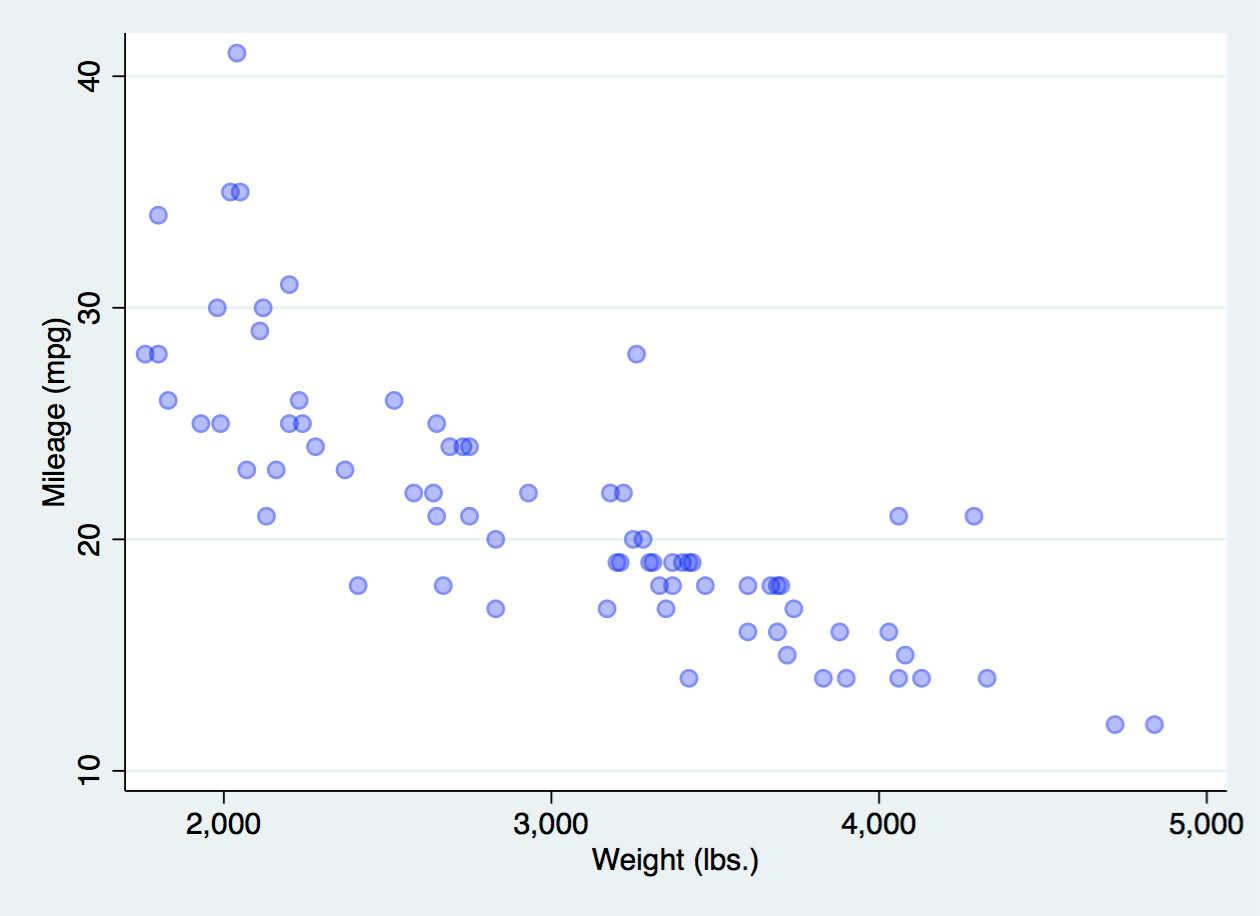
\includegraphics[height=4in]{graph.png}
\end{centering}
\end{center}

The .pdf file is generated with:

\begin{lstlisting}[frame=single]
dyntex extex.md, sav(extex.tex) replace
!pdflatex extex.tex
\end{lstlisting}

\end{document}

